\chapter{Metodología de desarrollo}
\label{cap:metodologia}

\section{Enfoque metodológico}
\label{sec:enfoque-metodologico}

El desarrollo de EpilexIA se llevó a cabo mediante un enfoque orientado a la
definición progresiva de requerimientos, el diseño e implementación de los
componentes del sistema y su posterior verificación y validación. Debido a que el proyecto se desarrolló en un contexto relacionado con el análisis de estudios EEG y comprendió la interacción de
diferentes componentes de \textit{software}, se consideró necesario mantener una correspondencia entre las necesidades identificadas, las funcionalidades implementadas y las actividades destinadas
a comprobar su funcionamiento.

Para organizar este proceso se adoptó como referencia el Modelo V de desarrollo
de sistemas. Este modelo permite relacionar las etapas de definición y diseño
con actividades posteriores de verificación y validación. En el proyecto, su
aplicación fue adaptada a las condiciones de trabajo existentes, particularmente
a la disponibilidad de los profesionales del área de Neurología del Hospital
Central del Instituto de Previsión Social y a la necesidad de presentar avances
funcionales durante las instancias de revisión.

\section{Modelo V}
\label{sec:modelo-v}

El Modelo V es un enfoque de desarrollo de sistemas que establece una relación
explícita entre las actividades de definición y diseño y las actividades de
verificación y validación. Su representación gráfica adopta la forma de una
letra V, en la que el lado izquierdo corresponde a la descomposición progresiva
del sistema desde los requerimientos hacia niveles de diseño más detallados,
mientras que el lado derecho representa las actividades de integración,
verificación y validación asociadas con los elementos definidos previamente
\citep{ForsbergMooz1991}.

Una característica fundamental del Modelo V es la correspondencia entre las
etapas de desarrollo y las actividades destinadas a comprobar los resultados
obtenidos. De esta manera, los componentes implementados pueden ser sometidos
a pruebas unitarias, su interacción puede evaluarse mediante pruebas de
integración y el sistema completo puede verificarse con respecto a los
requerimientos establecidos. Finalmente, la validación permite determinar si
la solución desarrollada responde a las necesidades y al propósito para los
cuales fue concebida \citep{ForsbergMooz1991}.

\section{Adaptación del Modelo V al proyecto \mbox{EpilexIA}}
\label{sec:adaptacion-modelo-v}

La aplicación del Modelo V en el desarrollo de EpilexIA se realizó de manera
adaptada a las características del proyecto y al contexto en el que se llevó
a cabo. Si bien se mantuvo como principio la correspondencia entre la
definición de requerimientos, el diseño de la solución, su implementación y
las actividades posteriores de verificación y validación, estas etapas no se
desarrollaron como una secuencia estrictamente lineal.

Una de las principales condiciones consideradas fue la disponibilidad de los
profesionales vinculados al proceso de análisis de estudios EEG en el Hospital
Central del Instituto de Previsión Social. Las instancias de interacción con
estos profesionales fueron utilizadas para relevar necesidades, revisar
funcionalidades y obtener retroalimentación sobre los avances realizados.
Como consecuencia, determinados requerimientos fueron precisados o ajustados
a medida que se disponía de nuevas observaciones sobre el funcionamiento del
sistema.

La validación incorporó además la revisión de avances funcionales y la
retroalimentación obtenida durante las instancias de seguimiento del proyecto.
Cuando estas revisiones evidenciaban nuevas necesidades o modificaciones sobre
una funcionalidad existente, los cambios se incorporaban nuevamente al ciclo
de análisis, diseño, implementación y verificación. De esta forma, el proyecto
mantuvo la relación entre las etapas planteadas por el Modelo V, pero permitió
iteraciones sobre determinadas partes del sistema cuando las condiciones del
desarrollo lo requerían.

\begin{figure}[H]
    \centering
    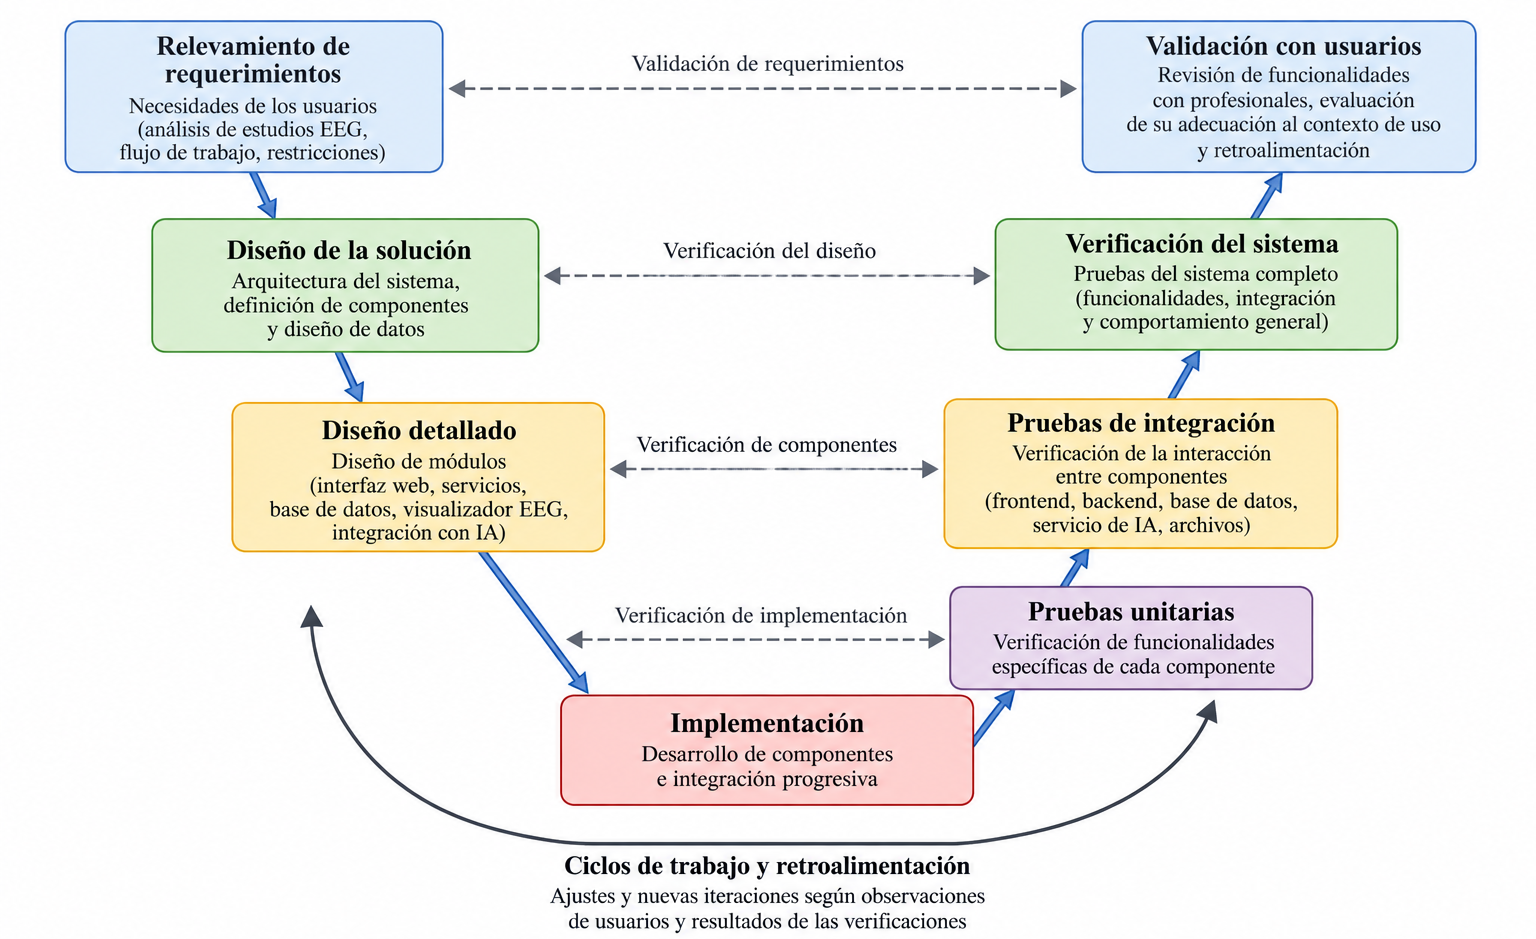
\includegraphics[width=\textwidth]{ThesisFigs/modelo_v_epilexia.png}
    \caption{Adaptación del Modelo V al proceso de desarrollo de EpilexIA.
    Elaboración propia basada en \citet{ForsbergMooz1991}.}
    \label{fig:modelo-v-epilexia}
\end{figure}

Esta adaptación del Modelo V al proceso de desarrollo de EpilexIA se
representa de forma esquemática en la Figura~\ref{fig:modelo-v-epilexia}.
La adaptación permitió conservar la trazabilidad entre las necesidades
identificadas, las decisiones de diseño, las funcionalidades implementadas y
las actividades destinadas a comprobarlas, sin impedir la incorporación de
retroalimentación durante el desarrollo. Las
secciones siguientes describen con mayor detalle las actividades de
relevamiento, diseño, implementación, integración, verificación y validación
realizadas en el proyecto.

\section{Relevamiento de requerimientos}
\label{sec:relevamiento-requerimientos}

El relevamiento de requerimientos constituyó una actividad fundamental para
comprender el contexto de utilización de EpilexIA y definir las funcionalidades
que debía proporcionar el sistema. Este proceso se desarrolló considerando el
flujo de trabajo relacionado con los estudios EEG en el Hospital Central del
Instituto de Previsión Social y las necesidades identificadas durante las
instancias de interacción con los profesionales involucrados.

Durante las primeras etapas del proyecto se analizaron las actividades
relacionadas con la gestión y revisión de estudios electroencefalográficos,
así como las características de las herramientas utilizadas en dicho contexto.
Este análisis permitió identificar necesidades vinculadas con el acceso a los
estudios, la visualización de señales EEG, la gestión de la información
asociada y la elaboración de informes, además de aspectos relacionados con la
seguridad, el control de acceso y la trazabilidad de las operaciones realizadas
en el sistema.

El relevamiento no se limitó a una única etapa inicial. A lo largo del
desarrollo se realizaron reuniones de seguimiento y revisión en las que se
presentaron avances funcionales y se analizaron observaciones sobre el
comportamiento esperado del sistema. Estas instancias permitieron precisar
requerimientos previamente identificados e incorporar ajustes derivados de una
mejor comprensión del flujo de trabajo y de las necesidades de los usuarios.

Los requerimientos relacionados con los perfiles de usuario también
evolucionaron durante el proyecto. Las primeras definiciones contemplaban una
separación más específica de determinados perfiles clínicos. Posteriormente,
a partir de las revisiones realizadas sobre el flujo de trabajo, estas
responsabilidades fueron reorganizadas en perfiles que representaran de forma
más adecuada la utilización prevista del sistema. Como resultado, la
configuración final contempla los perfiles Administrador, Técnico y
Especialista, cada uno asociado con las operaciones que le corresponden dentro
de EpilexIA.

\section{Diseño y desarrollo de la solución}
\label{sec:diseno-desarrollo-solucion}

A partir de los requerimientos identificados se inició el diseño de la solución,
definiendo los principales componentes de EpilexIA y las responsabilidades
asociadas con cada uno de ellos. El sistema fue concebido mediante una
arquitectura modular que permitiera separar la gestión de la información, la
lógica de negocio, la interacción con los usuarios y el procesamiento de las
señales EEG.

El diseño contempló una aplicación web para la interacción con los usuarios,
servicios de \textit{backend} encargados de gestionar la lógica del sistema y el acceso
a los datos, una base de datos para la persistencia de la información y
componentes destinados al procesamiento de los estudios EEG. Asimismo, se
consideró la integración con el servicio de inteligencia artificial encargado
del procesamiento automatizado de las señales, manteniendo separadas las
responsabilidades correspondientes a la aplicación web y al componente de
procesamiento mediante inteligencia artificial.

\section{Desarrollo asistido por inteligencia artificial}
\label{sec:desarrollo-asistido-ia}

La implementación de EpilexIA se realizó con la asistencia de herramientas de inteligencia artificial para la generación y revisión de código.
Los integrantes del equipo utilizaron Claude Code, Cursor y Codex, según la elección de cada desarrollador.

El equipo adoptó para los repositorios del sistema un conjunto de prácticas orientadas a mantener el control sobre el código producido:

\begin{itemize}
    \item \textbf{Contexto explícito por repositorio.}
    Cada repositorio incluye archivos que describen su arquitectura, sus convenciones y las reglas que deben respetar los asistentes (\texttt{CLAUDE.md}, \texttt{AGENTS.md} y reglas de Cursor).
    Estos archivos cumplen la función de documento rector del proyecto y permiten que distintos desarrolladores y herramientas trabajen sobre una base común.

    \item \textbf{Especificación y planificación previas.}
    El sistema cuenta con una especificación general, y los cambios de mayor alcance se elaboraron primero como planes documentados, que se conservan junto al código en la carpeta de documentación de los repositorios.

    \item \textbf{Revisión humana del código.}
    Los cambios se desarrollaron en ramas derivadas de la rama principal y se integraron mediante solicitudes de integración (\textit{pull requests}), revisadas por el líder técnico del equipo antes de su aprobación.

    \item \textbf{Verificación.}
    El código se acompañó de pruebas automatizadas y fue sometido a las actividades de verificación y validación que se describen en las secciones siguientes.
\end{itemize}

Esta forma de trabajo se relaciona con el desarrollo guiado por especificaciones, aunque no se adoptó una metodología formal de ese tipo.
Dentro del Modelo V, las prácticas descritas corresponden a las etapas de implementación y de verificación de componentes.
La asistencia de inteligencia artificial intervino en la producción del código, mientras que la definición de los requerimientos, las decisiones de diseño, la aprobación de los cambios y la validación con la especialista permanecieron a cargo del equipo.

\section{Verificación e integración}
\label{sec:verificacion-integracion}

La verificación de EpilexIA se realizó de manera progresiva durante el
desarrollo, con el propósito de comprobar que las funcionalidades
implementadas respondieran al comportamiento esperado antes de avanzar hacia
su integración con otros componentes. Este proceso permitió detectar
inconsistencias y realizar ajustes durante la construcción del sistema, en
lugar de concentrar las actividades de comprobación únicamente al finalizar
el desarrollo.

La integración con el subsistema de inteligencia artificial contempló
la solicitud de ejecuciones de procesamiento, su identificación y
seguimiento, la consulta de los estados correspondientes y la
recuperación de los resultados asociados con los estudios EEG.
Estas operaciones se verificaron mediante la ejecución del ciclo completo de procesamiento sobre estudios EEG reales, cuyos resultados se documentan en el Capítulo~\ref{pruebas_evaluacion}.

\section{Validación con usuarios}
\label{sec:validacion-usuarios}

Las actividades de validación funcional de EpilexIA comprendieron
instancias de revisión de las funcionalidades implementadas y la
obtención de retroalimentación de usuarios vinculados con el
contexto de utilización del sistema. Estas actividades permitieron
contrastar los avances realizados con las necesidades identificadas
durante el relevamiento y evaluar la adecuación de las
funcionalidades al flujo de trabajo previsto.

En particular, la validación se realizó con una médica especialista en epileptología del Hospital Central del IPS, mediante sesiones semanales desarrolladas en el hospital durante septiembre y octubre de 2026 sobre estudios EEG reales.
Las observaciones formuladas en dichas sesiones y su incorporación al sistema se detallan en el Cuadro~\ref{tab:observaciones-especialista}.

Las revisiones tuvieron especial importancia en las funcionalidades
relacionadas con el trabajo sobre estudios EEG. La disposición de los
elementos del visualizador, la representación de las señales, los controles
destinados al análisis y la organización de la información asociada al estudio
fueron objeto de ajustes durante el desarrollo. De manera similar, se revisaron
aspectos relacionados con los perfiles de usuario, la gestión de estudios, la
elaboración de informes y la presentación de los resultados provenientes del
procesamiento mediante inteligencia artificial.

Estas instancias de validación estuvieron orientadas principalmente a comprobar
la adecuación funcional y de uso de EpilexIA dentro del contexto para el cual
fue desarrollado. Por tanto, deben distinguirse de una validación clínica del
modelo de inteligencia artificial o de una evaluación destinada a establecer
la eficacia diagnóstica del sistema, aspectos que no forman parte del alcance
del presente trabajo.

\section{Ciclos de trabajo y retroalimentación}
\label{sec:ciclos-retroalimentacion}

El desarrollo de EpilexIA se organizó mediante ciclos de trabajo en los que
las actividades de análisis, diseño, implementación, verificación y revisión
se relacionaron de forma continua. Estos ciclos permitieron avanzar sobre
funcionalidades específicas y, al mismo tiempo, incorporar las observaciones
obtenidas durante las reuniones de seguimiento y las revisiones de los avances
del sistema.

En consecuencia, la adaptación metodológica utilizada en EpilexIA conservó la
relación entre requerimientos, diseño, implementación, verificación y
validación planteada por el Modelo V, incorporando ciclos de retroalimentación
cuando las revisiones funcionales o técnicas hacían necesario modificar una
decisión previa. Este enfoque permitió que la solución evolucionara de manera
controlada a partir de las necesidades identificadas y de los resultados
obtenidos durante su desarrollo.

